\documentclass[../mathNotesPreamble]{subfiles}

\providecommand{\relscalefact}{1.4}
\begin{document}
\relscale{\relscalefact}
  \section{8.3: Hypothesis Tests in Detail}
    \begin{defn*}[Type I and type II errors]
      \begin{itemize}
        \item A \textbf{type I error} is rejecting the null hypothesis, $H_0$, when it is actually true.
        \item A \textbf{type II error} is failing to reject the null hypothesis, $H_0$, when it is false.
      \end{itemize}
      The probability of committing a type I error is the level of significance: $\alpha$
    \end{defn*}
    \vspace*{\stretch{1}}

    \begin{center}
      \href[pdfnewwindow]{https://www.reddit.com/r/Mcat/comments/ao6ovi/type_i_and_type_ii_errors/}{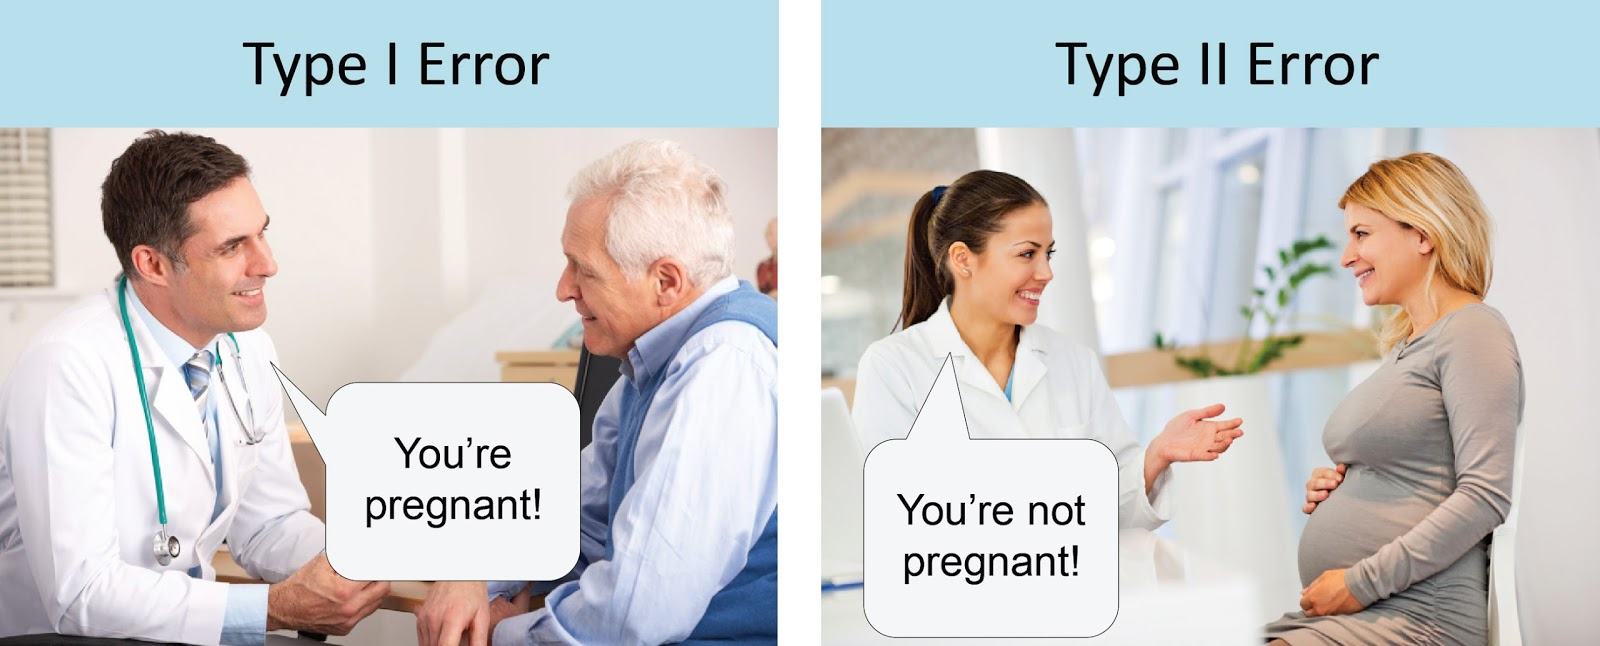
\includegraphics[width=0.85\linewidth]{images/Type_I_and_II_error.jpg}}
      \vspace*{\stretch{1}}

      \renewcommand{\arraystretch}{1.5}
      \begin{tabularx}{0.66\linewidth}{*{3}{@{}M{0.22\linewidth}@{}}}\toprule
        & Null Hypothesis \newline is true& Null Hypothesis \newline is false\\\midrule
        Reject null hypothesis& Type I error& True positive\\
        Fail to reject null hypothesis& True negative & Type II error\\\bottomrule
      \end{tabularx}
      \vspace*{\stretch{1}}
    \end{center}
  \pagebreak

  \begin{ex*}
    For the following scenarios, identify the type I and type II errors:
  \end{ex*}
  \begin{extasks}[after-item-skip=\stretch{1}](1)
    \task ``The Boy Who Cried Wolf''
    \task In a court of law, a person is considered innocent until proven guilty.
    \task Testing someone for a disease (e.g. Covid)
    \task Pregnancy test
  \end{extasks}
  \vspace*{\stretch{1}}
%  \pagebreak

  \fbox{\parbox{0.9875\linewidth}{
%    \textbf{Note:}
    \begin{itemize}
      \setlength{\itemsep}{0.75\baselineskip}
      \item When we ``fail to reject $H_0$'', we are \textbf{not proving} the null hypothesis
      \item Don't change your hypothesis after you gather your results
      \item Statistically significant means something likely did not occur by chance
      \item Confidence intervals vs. Hypothesis testing
        \begin{center}
          \begin{tabularx}{0.6\linewidth}{@{}*{2}{Y}@{}}\toprule
            Confidence Intervals& Hypothesis Tests\\\midrule
            Estimates parameters& Test parameters\\
            Range of values& Is data consistent?\\\bottomrule
          \end{tabularx}
        \end{center}
    \end{itemize}
  }}

  \pagebreak
\end{document}
